%%%%%%%%%%%%%%%%%%%%%%%%%%%%%%%%%%%%%%%%%
% Beamer Presentation
% LaTeX Template
% Version 1.0 (10/11/12)
%
% This template has been downloaded from:
% http://www.LaTeXTemplates.com
%
% License:
% CC BY-NC-SA 3.0 (http://creativecommons.org/licenses/by-nc-sa/3.0/)
%
%%%%%%%%%%%%%%%%%%%%%%%%%%%%%%%%%%%%%%%%%

%----------------------------------------------------------------------------------------
%	PACKAGES AND THEMES
%----------------------------------------------------------------------------------------

\documentclass{beamer}


\mode<presentation> {

% The Beamer class comes with a number of default slide themes
% which change the colors and layouts of slides. Below this is a list
% of all the themes, uncomment each in turn to see what they look like.

%\usetheme{default}
%\usetheme{AnnArbor}
%\usetheme{Antibes}
%\usetheme{Bergen}
\usetheme{Berkeley}
%\usetheme{Berlin}
%\usetheme{Boadilla}
%\usetheme{CambridgeUS}
%\usetheme{Copenhagen}
%\usetheme{Darmstadt}
%\usetheme{Dresden}
%\usetheme{Frankfurt}
%\usetheme{Goettingen}
%\usetheme{Hannover}
%\usetheme{Ilmenau}
%\usetheme{JuanLesPins}
%\usetheme{Luebeck}
%\usetheme{Madrid}
%\usetheme{Malmoe}
%\usetheme{Marburg}
%\usetheme{Montpellier}
%\usetheme{PaloAlto}
%\usetheme{Pittsburgh}
%\usetheme{Rochester}
%\usetheme{Singapore}
%\usetheme{Szeged}
%\usetheme{Warsaw}

% As well as themes, the Beamer class has a number of color themes
% for any slide theme. Uncomment each of these in turn to see how it
% changes the colors of your current slide theme.

%\usecolortheme{albatross}
%\usecolortheme{beaver}
%\usecolortheme{beetle}
%\usecolortheme{crane}
%\usecolortheme{dolphin}
%\usecolortheme{dove}
%\usecolortheme{fly}
%\usecolortheme{lily}
%\usecolortheme{orchid}
%\usecolortheme{rose}
%\usecolortheme{seagull}
\usecolortheme{seahorse}
%\usecolortheme{whale}
%\usecolortheme{wolverine}

%\setbeamertemplate{footline} % To remove the footer line in all slides uncomment this line
%\setbeamertemplate{footline}[page number] % To replace the footer line in all slides with a simple slide count uncomment this line

%\setbeamertemplate{navigation symbols}{} % To remove the navigation symbols from the bottom of all slides uncomment this line
}

\usepackage{amsmath,amssymb}
\usepackage{bm}
\usepackage{array}
\usepackage{tikz}
\usepackage{adjustbox}
\usepackage{ragged2e}
\usepackage{etoolbox}
\usepackage{graphicx} % Allows including images
\usepackage{booktabs} % Allows the use of \toprule, \midrule and \bottomrule in tables
\usepackage{bibentry}
%\usepackage[backend=biber,style=ieee, citestyle=authoryear]{biblatex}
\usepackage[style=ieee-alphabetic, backend=bibtex]{biblatex}



%\bibliography{bibfile.bib}
\addbibresource{bibfile.bib}



\makeatletter
\newcommand*{\mkblankfootnote}[1]{%
	\begingroup
	\renewcommand\thefootnote{}%
	\footnotetext{\bibfootnotewrapper{#1}}%
	\endgroup
}

\newcommand*{\mkbibsupercite}[1]{%
	\def\cbx@savedcites{\cbx@footfullcite}%
	\mkbibbrackets{#1}%
	\ifx\cbx@savedkeys\@empty
	\else
	\cbx@savedcites
	\fi}

\DeclareCiteCommand{\supercite}[\mkbibsupercite]
{\gdef\cbx@savedkeys{}}
{\usebibmacro{citeindex}%
	\usebibmacro{cite}%
	{}%
	\xappto\cbx@savedkeys{\thefield{entrykey},}}
{\supercitedelim}
{\protected@xappto\cbx@savedcites{%
		[\thefield{prenote}][\thefield{postnote}]{\cbx@savedkeys}}}

\DeclareCiteCommand{\cbx@footfullcite}
{}
{\mkblankfootnote{%
		\printtext[labelalphawidth]{%
			\usebibmacro{cite}%
		}%
		\setunit{\addspace}%
		\usedriver
		{\DeclareNameAlias{sortname}{default}}
		{\thefield{entrytype}}}}
{}
{}
\makeatother

\renewcommand*{\nameyeardelim}{\addcomma\addspace}

\apptocmd{\frame}{}{\justifying}{} % Allow optional arguments after frame.

\let\olditem\item
\renewcommand\item{\olditem\justifying}

\addtobeamertemplate{navigation symbols}{}{%
	\usebeamerfont{footline}%
	\usebeamercolor[fg]{footline}%
	\hspace{1em}%
	\insertframenumber/\inserttotalframenumber
}

%----------------------------------------------------------------------------------------
%	TITLE PAGE
%----------------------------------------------------------------------------------------

\definecolor{AtherosPrimary}{rgb}{0.992156,0.380392,0.34509803921}
\definecolor{AtherosSecondary}{rgb}{0.019,0,0.1568} % UBC Blue (primary)
\definecolor{AtherosTertiary}{rgb}{0.215,0.0625,0.515625}

\setbeamercolor{palette primary}{bg=AtherosSecondary,fg=white}
\setbeamercolor{palette tertiary}{bg=AtherosPrimary,fg=white}
\setbeamercolor{palette secondary}{bg=AtherosTertiary,fg=white}

\title{ETSI III} % The short title appears at the bottom of every slide, the full title is only on the title page

\logo{\includegraphics[width=1.2cm]{assets/sharif-logo.pdf}}


\author{Mohammad Raziei} % Your name
\institute[Sharif University] % Your institution as it will appear on the bottom of every slide, may be shorthand to save space
{
Sharif University of Technology\\ % Your institution for the title page
\medskip
\textit{mohammadraziei1375@gmail.com} % Your email address
}
\date{\today} % Date, can be changed to a custom date

\graphicspath {{images/}}

\newcommand{\mypause}{\pause}

\begin{document}

\begin{frame}
\centering
%\includegraphics[width=2cm]{sharif}
\titlepage % Print the title page as the first slide
\end{frame}

%----------------------------------------------------------------------------------------
%	PRESENTATION SLIDES
%----------------------------------------------------------------------------------------

\begin{frame}
	\frametitle{Researcher's Preface}
	
	I had studied \supercite{etsi1v1} and \supercite{etsi2v1} in previous meetings, and this week my focus is on \supercite{etsi3v1}.
	
	We will further become familiar with [ETS3], which focuses on system communication topics.
\end{frame}


\begin{frame}
    \frametitle{Overview} % Table of contents slide, comment this block out to remove it
    \tableofcontents 
\end{frame}




\section{Introduction to RIS}


\subsection{Definition of RIS}
\begin{frame}
	\frametitle{Definition of RIS}
	
	\begin{itemize}
	\mypause
	\item \textbf{It is a surface,} i.e. it is not a volumetric material, in order to reduce the implementation complexity, the losses,
	etc. while still being able to fully control the electromagnetic waves.
	\mypause
	\item\textbf{ It is an engineered (or intelligent) surface,} i.e. it can realize functions that a non-engineered surface (i.e. a
	metal plate) cannot realize.
	\mypause
	\item \textbf{It is reconfigurable,} i.e. its response can be adapted over time based on the network conditions. The
	reconfigurability encompasses multiple functions including controlled reflection, refraction, scattering,
	modulation, etc.
\end{itemize}
\end{frame}



\subsection{Types of RIS}
\begin{frame}
	\frametitle{Types of RIS}
	\begin{enumerate}\addtocounter{enumi}{0}
		\mypause
		\item \textbf{Reflecting surfaces:} This is an RIS that is capable of modifying the angle of reflection of an incident wave.
		\mypause
		\item \textbf{Refracting surfaces:} This is an RIS that is capable of modifying the angle of refraction (transmission) of an
		incident wave.
		\mypause
		\item \textbf{Joint reflecting and refracting surfaces:} This is an RIS that is capable of simultaneously modifying the
		angle of reflection and refraction of an incident wave.
		\mypause
		\item \textbf{Transmitting or information surfaces:} This is an RIS that is capable of encoding data and to realize singleRF (single-stream or multi-stream) transmitters. Examples include RIS that encode data onto the activations
		patterns of the unit cells or the synthetized radiation patterns.
	\end{enumerate}
\end{frame}

\begin{frame}
	\frametitle{Types of RIS}
	\begin{enumerate}\addtocounter{enumi}{4}
		\item \textbf{Surface for ambient backscattering:} This is an RIS that can simultaneously reflect or refract the incident
		waves and simultaneously modulate data onto the reflected or refracted wave.
		\mypause
		\item \textbf{Surfaced for tuned randomness:} This is an RIS that is configured in order to increase the scattering in a
		given area.
		\mypause
		\item \textbf{Absorbing surfaces:} This is an RIS that is configured to minimize the scattered field.
		\mypause
		\item \textbf{Communication and sensing surfaces:} This is an RIS with integrated communication and sensing capabilities, i.e. a surface that can simultaneously reflect a wave and detect the presence of objects.
	\end{enumerate}
\end{frame}


\subsection{Deployment scenarios}
\begin{frame}
	\frametitle{Deployment scenarios}
	
	\begin{itemize}\setlength\itemsep{1.5em}
		\item Enhanced connectivity and reliability
		\item Enhanced localization and sensing
		\item Enhanced sustainability and security
	\end{itemize}
\end{frame}


\section{Models for RIS}

\subsection{Models for radio localization and sensing}


\begin{frame}
	\supercite{gradoni2020endtoendmutualcouplingaware}
	
	\begin{figure}
		\centering
		\includegraphics[width=0.7\linewidth]{images/mutually-coupled}
		\caption{Mutually coupled antenna model}
		\label{fig:mutually-coupled}
	\end{figure}
\end{frame}


\begin{frame}

	
\begin{equation}
\scalebox{.77}{$
		\begin{array}{c}
		\bm{H} = \left( \bm{I}_{L_0} + \bm{\Psi}_{r,r} \bm{Z}_r^{-1} - \bm{\Psi}_{r,t} \left( \bm{\Psi}_{t,t} + \bm{Z}_t \right)^{-1} \bm{\Psi}_{t,r} \bm{Z}_r^{-1} \right)^{-1} \bm{\Psi}_{r,t} \left( \bm{\Psi}_{t,t} + \bm{Z}_t \right)^{-1} \\
		\bm{\Psi}_{t,t} = \bm{Z}_{t,t} - \bm{Z}_{t,S} \left( \bm{Z}_{S,S} + \bm{Z}_{tun} \right)^{-1} \bm{Z}_{S,t} \\
		\bm{\Psi}_{t,r} = \bm{Z}_{t,r} - \bm{Z}_{t,S} \left( \bm{Z}_{S,S} + \bm{Z}_{tun} \right)^{-1} \bm{Z}_{S,r} \\
		\bm{\Psi}_{r,t} = \bm{Z}_{r,t} - \bm{Z}_{r,S} \left( \bm{Z}_{S,S} + \bm{Z}_{tun} \right)^{-1} \bm{Z}_{S,t} \\
		\bm{\Psi}_{r,r} = \bm{Z}_{r,r} - \bm{Z}_{r,S} \left( \bm{Z}_{S,S} + \bm{Z}_{tun} \right)^{-1} \bm{Z}_{S,r}
	\end{array}
	$}
\end{equation}

\mypause

\begin{equation}
	\scalebox{.78}{$
\bm{H}_{r,t} \approx \left( \bm{I}_{L_0} + \bm{Z}_{r,r} \bm{Z}_r^{-1} \right)^{-1} \left( \bm{Z}_{t,t} + \bm{Z}_t \right)^{-1} \left( \bm{Z}_{r,t} - \bm{Z}_{r,S} \left( \bm{Z}_{S,S} + \bm{Z}_{tun} \right)^{-1} \bm{Z}_{S,t} \right)
	$}
\end{equation}
\end{frame}

\subsection{Localization}

\begin{frame}
	\frametitle{Technical Terms}
	\begin{table}[h!]
		\centering
		\begin{tabular}{lll}
			\toprule
			\textbf{Term} & \textbf{Abbreviation} & \textbf{Symbol} \\ 
			\midrule
			Signal Strength     & -                     & -               \\ 
			Time of Arrival     & ToA                   & $\tau$          \\ 
			Round-Trip Time     & RTT                   & -               \\ 
			Angle of Arrival    & AoA                   & $\theta$        \\ 
			Angle of Departure  & AoD                   & $\phi$          \\ 
			\midrule
			Single Input Single Output   & SISO                  & -               \\ 
			Multiple Input Single Output   & MISO                  & -               \\ 
			Single Input Multiple Output   & SIMO                  & -               \\ 
			Multiple Input Multiple Output   & MIMO                  & -               \\ 
			\bottomrule
		\end{tabular}
		\caption{Technical Terms}
	\end{table}
\end{frame}

\begin{frame}
	\frametitle{Localization scenarios}	

	\begin{figure}
		\centering
		\includegraphics[width=0.5\linewidth]{images/localization-scenarios}
		\caption{Localization scenarios}
		\label{fig:localization-scenarios}
	\end{figure}
\end{frame}


\begin{frame}
	\frametitle{SISO Localization}
	
	
	\supercite{Keykhosravi2022}
	
	
	
	\begin{minipage}{.6\linewidth}
		\begin{figure}
			\centering
			\begin{adjustbox}{scale=.4}
				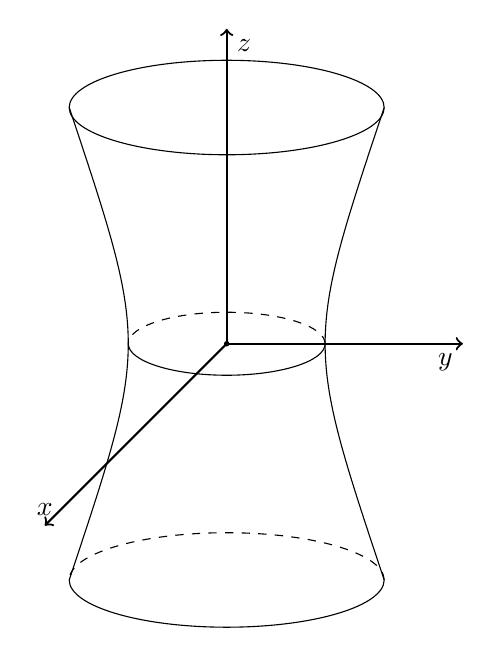
\begin{tikzpicture}
					% Draw the shaded hyperboloid with blue color
					
					% Outline of the hyperboloid's top and bottom circles
					\draw (0,3) ellipse (2cm and 0.6cm); % Top circle
					%		\draw (0,-3) ellipse (2cm and 0.6cm); % Bottom circle
					\draw[] (-2,-3) arc (180:360:2 and 0.6); % Solid visible arc at the equator
					\draw[dashed] (2,-3) arc (0:180:2 and 0.6);   % Dashed hidden arc at the equator
					
					% Draw the hyperboloid's connecting arcs
					\draw (-2,3) .. controls (-1,0) .. (-2,-3); % Left curve
					\draw (2,3) .. controls (1,0) .. (2,-3);    % Right curve
					
					% Draw the equator arcs (hidden and visible parts)
					\draw[] (-1.25,0) arc (180:360:1.25 and 0.4); % Solid visible arc at the equator
					\draw[dashed] (1.25,0) arc (0:180:1.25 and 0.4);   % Dashed hidden arc at the equator
					
					% Center point and radius line for reference
					\fill[fill=black] (0,0) circle (1pt); % Center point of the hyperboloid
%					\draw[dashed] (0,0) -- node[above]{$$} (1.25,0); % Radius line with label
					
							% Axes for reference
					\draw[thick,->] (0,0,0) -- (3,0,0) node[anchor=north east]{$y$};
					\draw[thick,->] (0,0,0) -- (0,4,0) node[anchor=north west]{$z$};
					\draw[thick,->] (0,0,0) -- (0,0,6) node[anchor=south]{$x$};
				\end{tikzpicture}
			\end{adjustbox}
			\caption{Hyperbolid:
			$\frac{x^2}{a^2} \pm \frac{y^2}{b^2} - \frac{z^2}{c^2} = 1$
			}
		\end{figure}
	\end{minipage}\hfill
	\begin{minipage}{.3\linewidth}
		\begin{figure}
			\centering
			\includegraphics[height=0.4\paperheight]{images/siso-1}
			\caption{1 RIS, 1 BS, WB}
			\label{fig:siso-1}
		\end{figure}
	\end{minipage}
\end{frame}

\begin{frame}
	\frametitle{SISO Localization}
	\begin{minipage}{.6\linewidth}
		\begin{figure}
			\centering
			\begin{adjustbox}{scale=.6}
				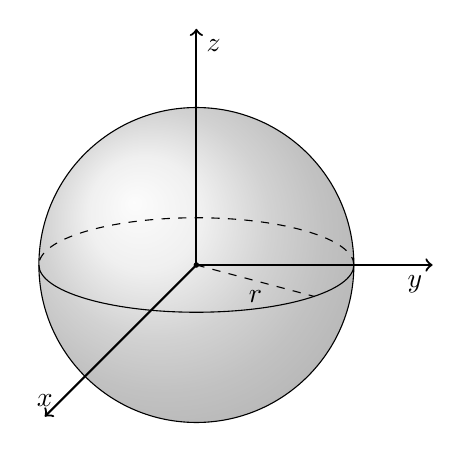
\begin{tikzpicture}
					\shade[ball color = gray!40, opacity = 0.4] (0,0) circle (2cm);
					\draw (0,0) circle (2cm);
					\draw (-2,0) arc (180:360:2 and 0.6);
					\draw[dashed] (2,0) arc (0:180:2 and 0.6);
					\fill[fill=black] (0,0) circle (1pt);
					\draw[dashed] (0,0) -- node[below]{$r$} (1.5,-.4);
					
												% Axes for reference
					\draw[thick,->] (0,0,0) -- (3,0,0) node[anchor=north east]{$y$};
					\draw[thick,->] (0,0,0) -- (0,3,0) node[anchor=north west]{$z$};
					\draw[thick,->] (0,0,0) -- (0,0,5) node[anchor=south]{$x$};
				\end{tikzpicture}
			\end{adjustbox}
			\caption{Sphere:
				${x^2} + {y^2} + {z^2} = r^2$
			}
		\end{figure}
		
	\end{minipage}\hfill
	\begin{minipage}{.3\linewidth}
		\begin{figure}
			\centering
			\includegraphics[height=0.4\paperheight]{images/siso-2}
			\caption{1 RIS, 0 BS, WB}
			\label{fig:siso-2}
		\end{figure}
	\end{minipage}
\end{frame}


\begin{frame}
	\frametitle{SISO Localization}
	\begin{minipage}{.6\linewidth}
		

		
	\end{minipage}\hfill
	\begin{minipage}{.4\linewidth}
		\begin{figure}
			\centering
			\includegraphics[height=0.4\paperheight]{images/siso-3}
			\caption{2 RIS, 0 BS, NB}
			\label{fig:siso-3}
		\end{figure}
	\end{minipage}
\end{frame}



\begin{frame}
	\frametitle{MISO Localization}
	\begin{minipage}{.5\linewidth}
		
		
		
	\end{minipage}\hfill
	\begin{minipage}{.45\linewidth}
		\begin{figure}
			\centering
			\includegraphics[height=0.4\paperheight]{images/miso}
			\caption{1 RIS, 1 BS, NB}
			\label{fig:miso}
		\end{figure}
	\end{minipage}
\end{frame}




\begin{frame}
	


\end{frame}



\begin{frame}[allowframebreaks]
\frametitle{References}
    \printbibliography
\end{frame}

%----------------------------------------------------------------------------------------

\end{document} 

